\section{\textbf{Work Plan}}\label{sec:conclusions}


%-------------------------------------------------------------------------------
%In general a short summarizing paragraph will do, and under no circumstances
%should the paragraph simply repeat material from the Abstract or Introduction.
%In some cases it's possible to now make the original claims more concrete,
%e.g., by referring to quantitative performance results.

%The further work material is important -- part of the value of a paper is
%showing how the work sets new research directions. (1) If you're actively
%engaged in follow-up work, say so. E.g.: "We are currently extending the
%algorithm to... blah blah, and preliminary results are encouraging." This
%statement serves to mark your territory. (2) Conversely, be aware that some
%researchers look to Future Work sections for research topics. 

%This section should summarize what has  been accomplished in the paper. Many
%readers will read only the Introduction and Conclusion of your paper. The
%Conclusion should be written so they can be understood by someone who has not
%read the main work of the paper.

%-------------------------------------------------------------------------------
%We have shown that\dots. The crucial results are\dots.  
%-------------------------------------------------------------------------------
 
The 5G-TSN integration is a crucial topic of importance for all communication companies.The 5G and TSN mixture is ideal for intelligent factories, given ultra-reliability and low latency characteristics. Although, a particular level of integration of the couple technologies is required to present End-to-End Ethernet connectivity to match the industrial requirements. That allows us to imagine; How much the integrated time synchronization through wired TSN and wireless 5G domains affords a regular reference time for industrial endpoints. 5G is also integrated with the given TSN tool used in an unusual deployment to accommodate limited low latency. End-to-End Ultra-reliability and high availability are granted by the arrangement of the disjoint forwarding paths of the 5G and TSN segments \cite{Ericsson2019}. This study aims to understand the open-source 5G core Network benefits and Time-sensitive Network (TSN) features. The integration between both technologies is the key To achieve eMBB,  mMTC, and uRLLC. In this Thesis, we tried to design and implement the best effort testbed environment that can be provided by integrating open source 5GC and TSN. Chapter 2 (State of the Art) in the thesis paper can give us all the background that we need to understand this thesis. It provides more knowledge about architecture. In addition to that, we will also deploy a Standalone 5GC Network.
Chapters 4, 5, and 6 (Design and Specifications) explain the implementation's needed knowledge in detail.
Last but not least, Wireshark and Iperf are utilized to achieve a Comparative Analysis of OS 5G Core Implementations and Design and Evaluation of a 5G Testbed.



%\sidenote{results}
%\todomid{We have shown that\dots}.
%\todomid{The crucial results are\dots.}

%-------------------------------------------------------------------------------
%Recipient of the results/improvements. Who gaines provit from this?
%-------------------------------------------------------------------------------
%\sidenote{benefits}
%\todomid{The presented work provides %potential benefits for\ldots}

%-------------------------------------------------------------------------------
%Further work: start with short-term, then long-term ojectives.
% -------------------------------------------------------------------------------



%\subsection{Enhancement of hardware-supported scheduled TSN traffic (out of scope of this thesis)}\label{Enhancement of hardware-supported scheduled TSN traffic (out of scope of this thesis)}
%\subsection{Integration of hardware-supported scheduled TSN traffic (out of scope of this thesis)}\label{Integration of hardware-supported scheduled TSN traffic (out of scope of this thesis)}

%\subsection{Summary}\label{Summary}
%\subsection{Conclusion and Future Work}\label{Conclusion and Future Work}


\subsection{\textbf{Thesis Structure}}\label{Structure of the Thesis} 



 
\begin{figure}
Thesis Structures illustrated in figures \textbf{\ref{fig:Thesis-TOC1}},\textbf{\ref{fig:Thesis-TOC2}},\textbf{\ref{fig:Thesis-TOC3}},\textbf{\ref{fig:Thesis-TOC4}},


 \end{figure}
\begin{figure}
 
\centering
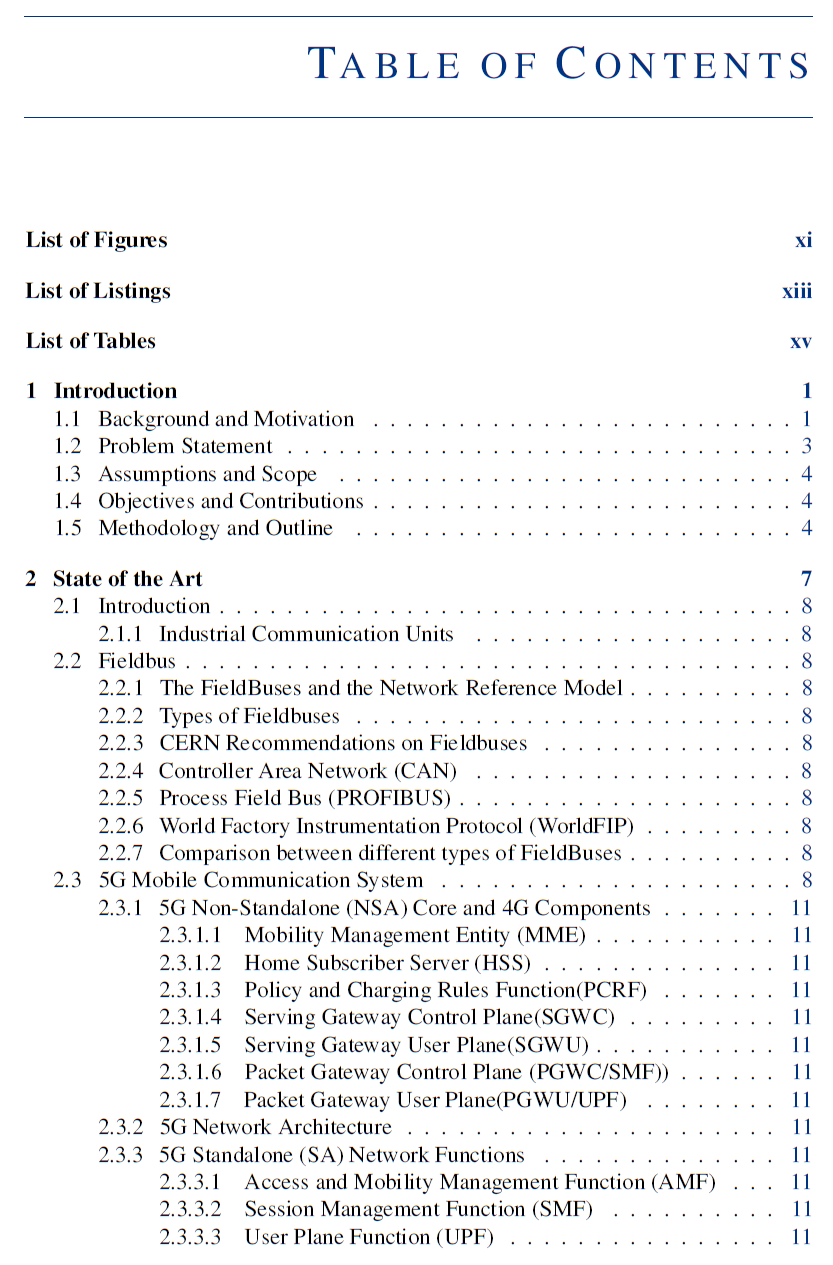
\includegraphics[scale=0.41]{images/Thesis-TOC1.png} 
\caption{Thesis Structure TOC1}
\label{fig:Thesis-TOC1}
 

 \end{figure}
\begin{figure}

 
  \centering
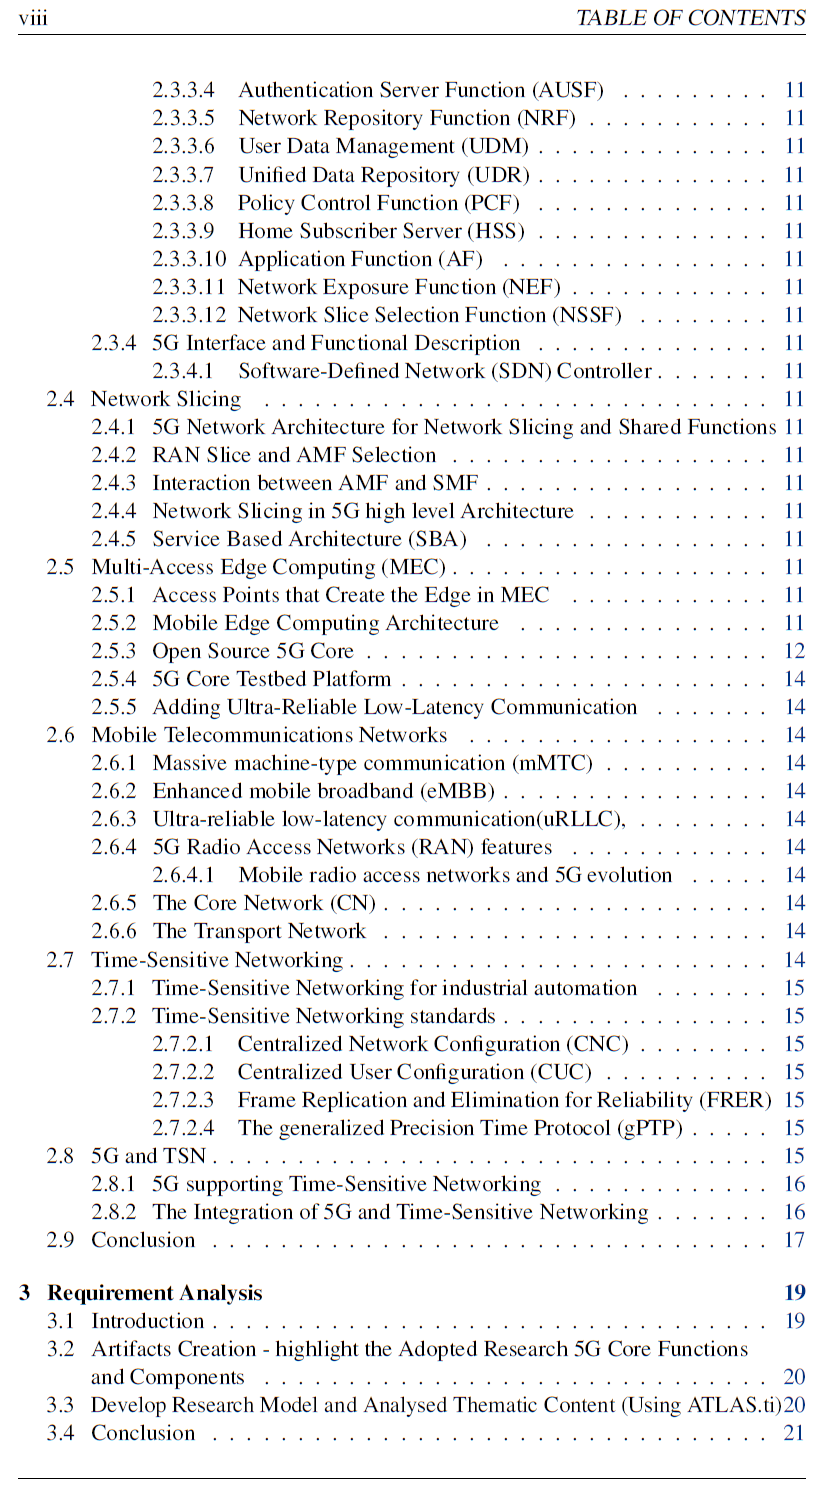
\includegraphics[scale=0.39]{images/Thesis-TOC2.png} 
\caption{Thesis Structure TOC2}
\label{fig:Thesis-TOC2}
 \end{figure}
 
 
 
\begin{figure}
\centering
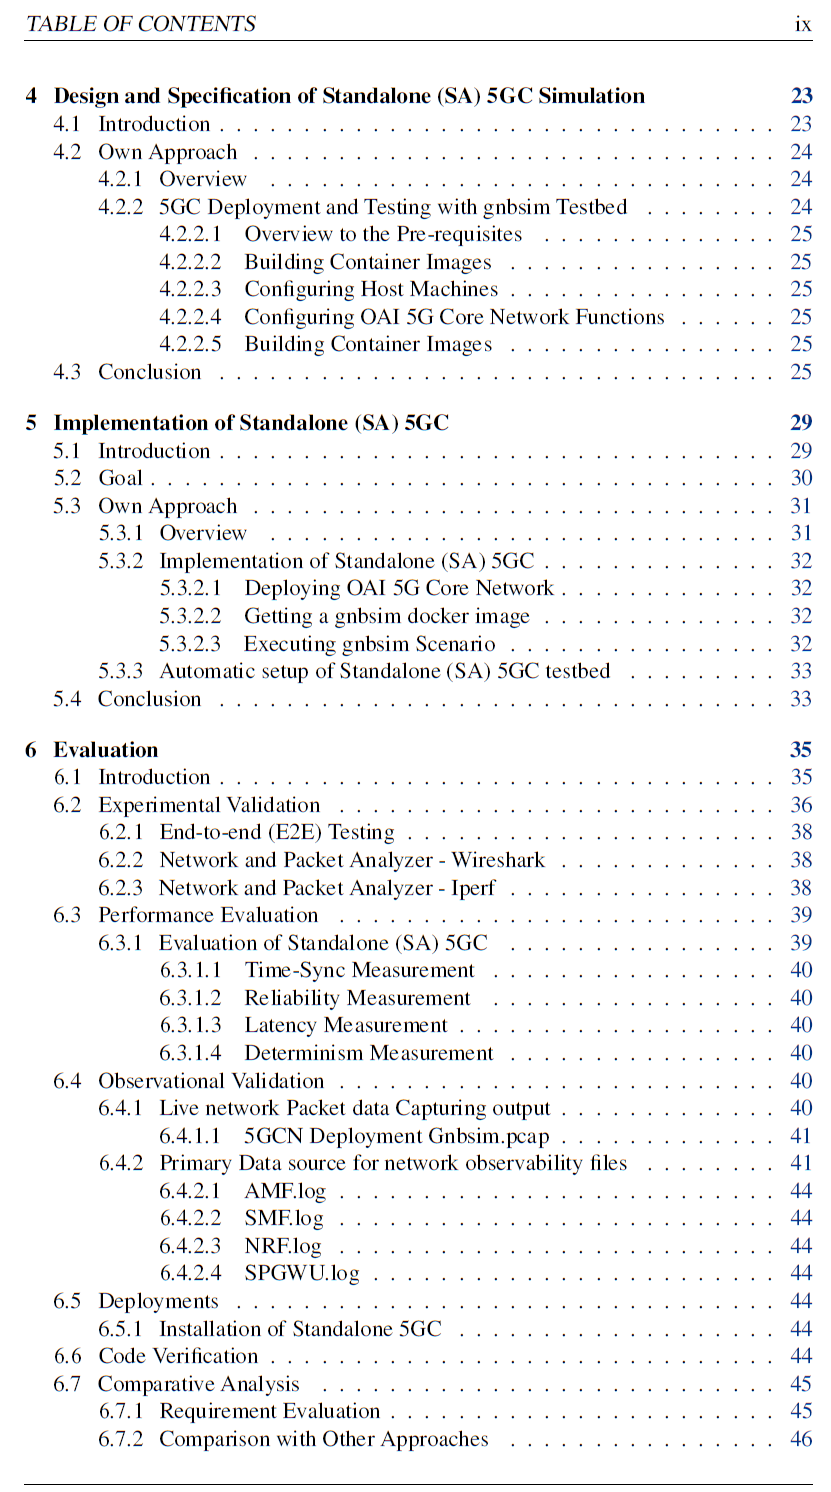
\includegraphics[scale=0.41]{images/Thesis-TOC3.png} 
\caption{Thesis Structure TOC3}
\label{fig:Thesis-TOC3}
 \end{figure}
 
\begin{figure}
\centering
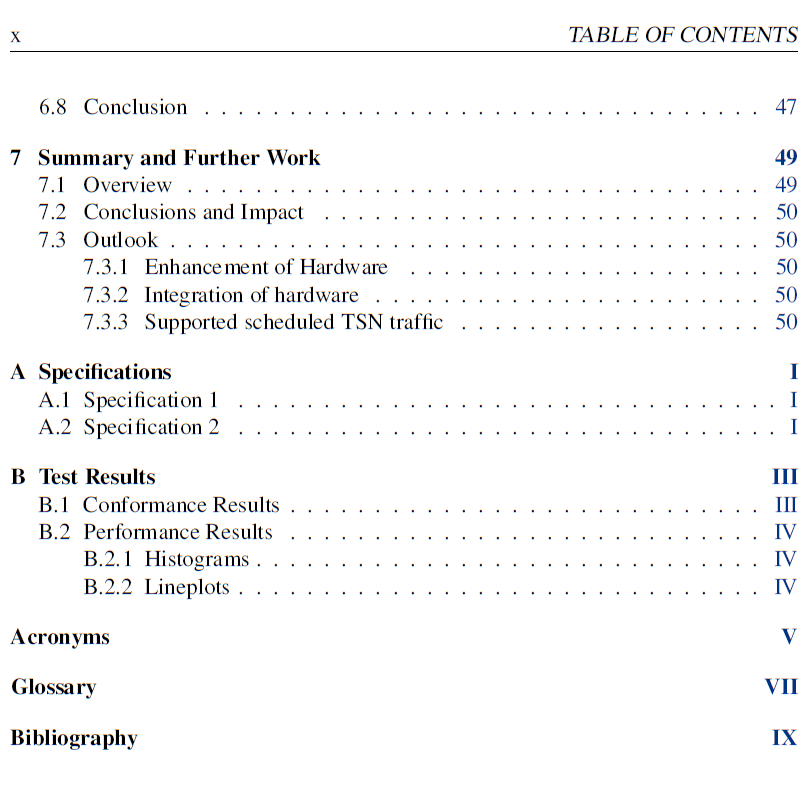
\includegraphics[scale=0.40]{images/Thesis-TOC4.png}
\caption{Thesis Structure TOC4}
\label{fig:Thesis-TOC4}
 \end{figure}
 
\clearpage


\subsection{\textbf{Gantt}}\label{Gantt timeline- with milestones and overall planned duration}

As mandate by Regulations Governing General Study and Examination Procedures (AllgStuPO), the period to work for a master thesis should be in six months.
The proposed timeline to commence this work is depicted in figure \textbf{\ref{fig:Thesis_High-level_Timeline}}
below.
 
 
 
\begin{figure}
 
\centering
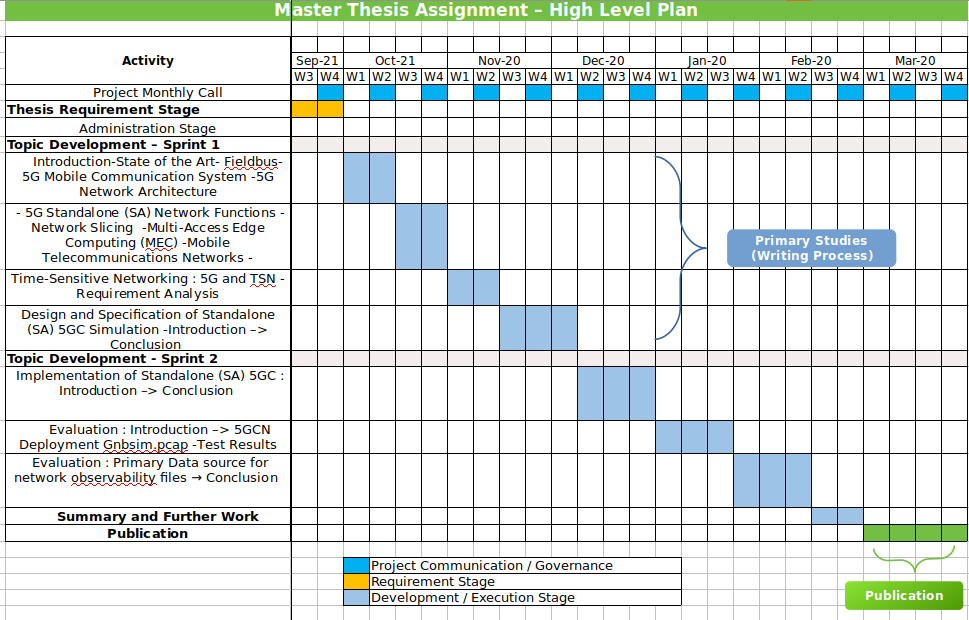
\includegraphics[scale=0.35]{images/Timeline_OS_5GC.png}
\caption{Master Thesis High level Timeline.}
\label{fig:Thesis_High-level_Timeline}
  \end{figure}

 
%\sidenote{gap 2}
%\todotext{related work 2}

%\sidenote{gap 3}
%\todotext{related work 3}

%\sidenote{issue}
%\todotext{outstanding problem}

